\documentclass{article}
\usepackage[utf8]{inputenc}
\usepackage[spanish]{babel}
\usepackage{listings}
\usepackage{graphicx}
\graphicspath{ {images/} }
\usepackage{cite}

\begin{document}

\begin{titlepage}
    \begin{center}
        \vspace*{0.5cm}
            
        \Huge
        \textbf{Memoria}
            
        \vspace{0.5cm}
        \LARGE
        Informática II
            
        \vspace{1.5cm}
            
        \textbf{José Alfredo Solano Lorduy}
        
        \vspace{2.5cm}
        
        \begin{figure}[h]

\includegraphics[width=4cm]{Udea.png}
\centering
\caption{Logo de UdeA}
\label{fig:udealogo}
\end{figure}
            
        \vfill
            
        \vspace{0.8cm}
            
        \Large
        Despartamento de Ingeniería Electrónica y Telecomunicaciones\\
        Universidad de Antioquia\\
        Medellín\\
        Septiembre de 2020
            
    \end{center}
\end{titlepage}

\tableofcontents

\section{Introducción}
Para introducir un poco mas en contexto, es pertinente conocer el significado de las siglas RAM, su forma física a modo de guía y su tarea principal. RAM son las siglas de «Random Access Memory» o «Memoria de Acceso Aleatorio». Su formato más extendido es el de un PCB a modo de pastilla rectangular sobre el que se asientan diferentes chips que contienen cantidades determinadas de memoria RAM, su labor principal, se basa en cargar archivos de forma rápida para que el procesador (CPU) ejecute dichos archivos y poder interactuar de forma efectiva con nuestro sistema.\cite{muycomputer}

\section{Contenido} \label{contenido}
\vspace{0.5cm}
\subsection{Definición de memoria}
La memoria del computador es uno de los elementos más importantes del sistema, en palabras generales, su funcionalidad es almacenar, cargar, enviar y recibir la información contenida por esta misma, con la cual se realizan distintos tipos de interacciones o cambios. Hay distintos tipos de memorias para distintas tareas, la velocidad de transferencia de información varía dependiendo el grado de necesidad que el sistema necesite.
\vspace{0.5cm}
\subsection{Tipos de memoria}
Dentro de mis conocimientos propios, conozco tres tipos de memorias:
\subsubsection{Memoria RAM}
Complementando la infomación anteriormente expuesta, se encarga de cargar las aplicaciones, programas y archivos desde la memoria secundaria y mantenerlos abiertos de forma rápida.
\subsubsection{Memoria de almacenamiento secundaria}
Conocido también como disco duro, se encarga de almacenar el sistema operativo, los archivos y programas que este contenga, sus velocidades varían de acuerdo a la interfaz que se use.
\subsubsection{Memoria caché}
La memoria caché según mis conocimientos, se ubica físicamente en el procesador, su función es almacenar información que puede serle útil al sistema para acceso de manera muy rápída.
\vspace{0.5cm}
\subsection{¿Cómo se gestiona la memoria?}
Ya que conocemos el significado, la función y la forma física de la memoria, la gestión es lo más importante al momento de usarla, se le llama gestión de memoria al acto de gestionar la memoria de un computador o sistema infomático. En pocas palabras, se trata de brindar alternativas para asignar secciones de memoria a los programas que las solicitan, y a la vez, liberar las secciones de memoria que ya no se utilizan para que estén disponibles para otros programas.\cite{gestion}
\vspace{0.5cm}
\subsection{Velocidad de las memorias y su importancia}
Las velocidades de las memorias varían de acuerdo a las necesidades y las exigencias de los sistemas en los que trabajamos, cada memoria tiene distinta frecuencia y distinta velocidad de transferencia.
\subsubsection{RAM}
La memoria ram interactúa directamente con el procesador, utiliza distintas frecuencias de acuerdo a las tecnologías usadas, existen varias mejoras que se les denominan DDR (Double Data Rate) que hacen dos tareas de lectura y dos tareas de escritura por cada ciclo del reloj, las frecuencias varían desde los 667 MHz (Megahercios) hasta los 3600 MHz, esto depende de el tipo DDR que usemos. Las velocidades de transferencia oscilan entre los 16gb/s (gigabytes por segundo) y pueden llegar mucho más lejos. La importancia de estas velocidades son para lograr cargar las aplicaciones, archivos y ejecutables del sistema operativo (incluyendo el mismo sistema) de manera rápida y amigable para el usuario.\cite{velocidadram}
\subsubsection{Disco duro o memoria de almacenamiento}
La memoria secundaria, tiende a tener velocidades bastante más bajas que la memoria RAM, esto porque no es del todo necesario. El disco duro no interacciona directamente con el procesador, utiliza la RAM como intermediario y por tanto, la información se transfiere de manera más lenta. Las velocidades de los discos mecánicos varía entre los 100 mb/s (megabytes por segundo) y los 300 mb/s, los discos modernos de estádo sólido, llegan a tener velocidades de 5gb/s.\cite{DiscoDuro}
\subsubsection{Memoria Caché}
La memoria caché es la que tiene menos capacidad de todas, mas sin embargo, su velocidad de transferencia está por los 1150 gb/s, siendo la memoria de acceso más rápida que se encuentra en nuestro equipo.\cite{cache}

\vspace{1.5cm}




Imagen de la memoria RAM Figura (\ref{fig:RAM})

\begin{figure}[h]
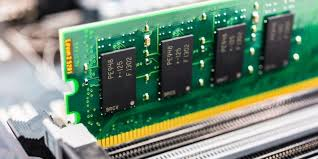
\includegraphics[width=4cm]{Random access memory.jpg}
\centering
\caption{Memoria Ram}
\label{fig:RAM}
\end{figure}
\cite{Memory}

\section{Conclusión} \label{conclulsion}
En conclusión, la memoria es un elemento vital para el funcionamiento de un equipo, sus tareas van desde el manejo de datos, almacenamiento, transferencia y la interacción humano - computador de un sistema informático, las diferencias en las memorias están marcadas principalmente para ser utilizadas con distintas finalidades, dependen de las tareas y operaciones básicas que el sistema deba realizar. Las capacidades son limitadas actualmente y con ayuda de las nanotecnologías, estas capacidades llegarán a ser bastante mayores sin necesidad de ocupar tanto espacio físico.
\bibliographystyle{IEEEtran}
\bibliography{references}

\end{document}
